%%% Template for the submission to  %%%
%%%     Binghamton University CS480/580  (ndjfl)
%%%
%%% Usage summary %%%
%%%     Mostly, the information
%%%     required is obvious, but some explanations are given.
%%%     All other lines should be ignored.  

\documentclass{ndjflart}
%%% HIGHLY RECOMMENDED PACKAGES AND SETTINGS
%\usepackage{pdfsync}  %% if you know what this is use it or not. 
\usepackage[T1]{fontenc}
%%%%%%%%%%%%%%%%%%%%%%%%%%%%%%
%% If your tex system is less than 2 years old (in 2012) the following
%% font options are available. If not comment them out.
\usepackage{graphicx} % Required for including images
\usepackage{tgtermes}
%       otherwise use alternative journal fonts
%\renewcommand{\rmdefault}{ptm} % system default Times font
\usepackage{mathptmx}  
%%%     additional fonts
\usepackage[scaled=.92]{helvet}
%\setoptfont{enc={T1},fam={pop}} % if You have Optima font, uncomment this line
%%% MATH
\usepackage{amsthm,amsmath,amssymb}
\usepackage{mathrsfs}
%%% BIBLIOGRAPHY
\usepackage[numbers]{natbib}  %% numbers is required.
%%% LINKS
\usepackage[colorlinks,citecolor=blue,urlcolor=blue]{hyperref}  %%check

\artstatus{am} %%% leave this alone!!  That means you, too!!
%%%%%%%%theorems%%%%%


%%%% feel free to changes these%%%%%%%
\newtheorem{theorem}{Theorem}[section]
\newtheorem{lemma}[theorem]{Lemma}
\newtheorem{conjecture}[theorem]{Conjecture}
\newtheorem{condition}[theorem]{Condition}
\newtheorem{claim}[theorem]{Claim}
\newtheorem{question}[theorem]{Question}
\newtheorem{corollary}[theorem]{Corollary} 
\theoremstyle{definition}
\newtheorem{definition}[theorem]{Definition}
\newtheorem{statement}[theorem]{Statement}
\newtheorem{notation}[theorem]{Notation} 
\theoremstyle{remark}
\newtheorem{remark}[theorem]{Remark}



%%%DATE enter the date of your submission here- best%%%
%%%If \date{} is not used, the current date will be used%%%
%%%Warning:This will be lost if your paper is recompiled on another day though%%%
%%%\date{May 30, 2012}%%%%
\date{October 10, 2019}

%%%PUT YOUR DEFINITIONS HERE%%%
%NDJFL uses \varphi by default; redefine only if you want \phi%%%

\startlocaldefs
%%% our macros for this article only %%%%
\newcommand{\NDJFL}{\emph{NDJFL}}
\newcommand{\Jo}{\emph{Journal}}
\newcommand{\EM}{Editorial Manager}
\newcommand{\origphi}{\phi}
\newcommand{\CMS}{\emph{CMS}}
\newcommand{\mn}{\medskip\noindent}
\newcommand{\tietilde}{\char126\relax}

\endlocaldefs

\begin{document}

\begin{frontmatter}

  %% TITLE OF YOUR PAPER%%%
  %% Words in title should begin with uppercase, except%%%
  %%% articles (and, the, a), conjunctions (and, for, nor, but),
  %%% prepositions (by, with, for, over, and so on)
  \title{\emph{Development of Human Following}\\
    \emph{Mobile Robot System Proposal}}
  %%% Choose a short title to be used as the running head on
  %%% odd-numbered pages%%%
  %%% Use this same title as "short title" when you submit MS to
  %%% EM%%%%
  \runtitle{Human Following Mobile Robot System}

  \author{\fnms{Emily} %first name
    \snm{Lakic}%last name
    \corref{}%to denote who is the corresponding author
    \ead[label=e1]{elakic1@binghamton.edu}%author email, leave this [label] as is
    \ead[label=u1,url]{}%%web page, leave this [label] as is
  }
  %%% ADDRESS NOTES
  %%% Dept listed first, University/company second, street or PO box
  %%% third%%%
  %%% U.S. Postal Service guidelines request no punctuation in the
  %%% street...country lines%%%
  %%% Country should be all uppercase%%%%
  \address{Computer Science Department\\
    Binghamton University\\
    4400 Vestal Parkway East\\
    Binghamton NY 13902\\
   USA\\
    \printead{e1}\\
    \printead{u1} }%
  \and%
  \author{\fnms{Umut}
    \snm{Kayaalti}\ead[label=e2]{ukayaal1@binghamton.edu}}%increase label by
  %	% one for each
  %	% author
  \address{Computer Science Department\\
    Binghamton University\\
    4400 Vestal Parkway East\\
    Binghamton NY 13902\\
    USA\\
    \printead{e2} }
  % \and \author{\fnms{???} \snm{???}\ead[label=e3]{???}}
  % \address{\printead{e3}} \affiliation{???}

  %%%% INSERT EACH AUTHOR'S FIRST INITIAL AND SURNAME%%%%
  \runauthor{E.~Lakic and U.~Kayaalti}


\begin{abstract}
 A human-following robot has plenty of applications in daily life and manufacturing. Autonomous robots can learn to 'follow the leader' in an effort to provide as mission partners for humans, whether to assist in day-by-day tasks or for more extensive use as industrial robots operating in complex environments. The purpose of the development of a human following mobile robot system is to provide a robot the ability to actively follow a person while keeping a certain distance. If that person moves away, the robot will move until the person is as close as the specified distance again, or will rotate to keep him/her in its lenses. Robotic vision tools will operate vastly from the generation of robot movement through sensor and detection algorithm inputs, to  the use of rapid RGB image processing and open source computer vision libraries to detect human activity. A more complex analysis of the distance between the robot and said human will be measured by a ros scan.
  
\end{abstract}

\begin{keyword}[class=AMS]
  \kwd[Primary ]{X001} \kwd{Y002} \kwd[; Secondary ]{Z003}
\end{keyword}

\begin{keyword}
  \kwd{typesetting} \kwd{guide for authors}
\end{keyword}

\end{frontmatter}

% main matter with bibliography goes here

\section{Technical Details}\label{intro}

Making the robot detect a human and then actively follow them will heavily require us to rely on robot vision tools. To make robots detect human will require libraries from open source computer vision library called opencv. There are different pre-trained models and methods to detect humans from histogram of oriented gradients and haar cascade to more convolutional neural network based approaches with tensorflow detection zoo library. While this rapid image processing part will be in RGB there will most likely be needed to use ros scan to determine the distance towards the detected object/human. The movements of the robot will be based on the inputs it will receive from these sensors and detection algorithms. As for the following and movement parts of the robot will most likely handwritten.

\begin{center}
	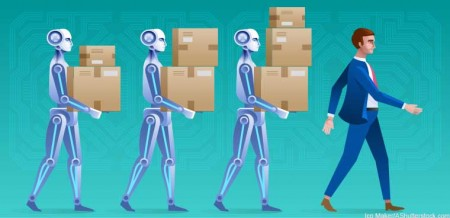
\includegraphics[width=0.5\columnwidth]{robotsfollowhuman-450x218.jpg} % Example image
\end{center}

\section{Potential Challenges}\label{front}
While following the human, the robot will have to avoid obstacles on its path. Another thing to note is that the human won’t be always moving predictably, such as moving in a straight line. There will be erratic movements, such as sudden stops, change of direction, and angular movements and through these, the robot should be able to assess and act accordingly to keep the human inside its sights. Finally, there will be times where the human will go missing from the robots perspective. This will require the robot to actively search for and get him or her back in its radar.

\section{Success Criteria}\label{secs} We will measure the success of our robot by how accurately the robot can detect the human, how long the robot can keep following the human in its environment without losing track of him/her in a increasingly more erratic movement patterns, and finally how often it can find the human that it lost track of.


\section{Motivation}\label{style} 

Motivation for a human following mobile robot system adhered to developing a robot capable of socially appropriate spatial skills not only to travel the path of a human but to accompany and go as far as aid the individual. Though medicinal practice has reached a breakthrough in recent years, there is nonetheless a number of elderly individuals in need of support through their day-by-day activities. A cost and time efficient means to providing aid may be achieved through the use of a mobile robot system. As many people are not roboticists, we consider the fact that our robot must move in ways easy to understand and socially acceptable to individuals.  


\section{Work Distribution}\label{gandt} 
Work completed on our project will be divided into two to adequately distribute tasks among group members. Image processing and ros scan will be implemented by both team members as it will both help with direction and with robotic vision.

\subsection{Emily}\label{sseccommas} 
Emily will focus on the mobility of the robot. As aforementioned, it is important to note that many are not accustomed to working with robots and thus the robot must be programmed in a way that is easy to understand and will navigate in a path that is comfortable to the human to build a sense of trust.

\subsection{Umut}\label{sseclabel} 
Umut will focus on the vision aspects of the robot based on convolutional neural network approaches as well as exploring libraries, such as that from the open source computer vision library. 


\section{Past Research}\label{ams}
Human following robots have been researched and developed actively in the past few decades. Previous research has explored several techniques such as human’s target detection, robot control algorithm, and obstacles avoidance. Various approaches have been followed, including the use of ultrasonic, voice recognition, and laser range sensors, as well as a charge-coupled device (CCD) camera, and so on. In the study \textit{Natural Person-Following Behavior for Social Robots}, Rachel Gockley, Jodi Forlizzi, and Reid Simmons of Carnegie Mellon University looked to combine technological aspects with social psychology and interaction design, to develop robots that can accompany people in socially acceptable ways. Such approaches were explored as possibilities prior to beginning research and development into our project. 


%\bibliographystyle{jflnat} 
%\bibliography{GTA}

%%% ACKNOWLEDGMENTS= your personal comments and thanks %%%


\end{document}


%%%%%%%%%%%%%GTA.bib%%%%%%%%%%
@book{CMS,
	EDITOR = {University of Chicago Press Staff},
	TITLE = {The Chicago Manual of Style},
	PUBLISHER = {The University of Chicago Press},
	ADDRESS = {Chicago},
	YEAR  = {2010},
	EDITION = {16th}
}

@book{copy,
	TITLE = {Butcher's {C}opyediting: {T}he {C}ambridge {H}andbook for {E}ditors, {C}opyeditors and {P}roofreaders},
	AUTHOR = {Judith Butcher},
	PUBLISHER = {Cambridge University Press},
	ADDRESS = {Cambridge},
	YEAR = {1981},
	EDITION = {4th}
}

@article{ghma09,
	AUTHOR = {Gherardi, Guido and Marcone, Alberto},
	TITLE = {How incomputable is the separable {H}ahn-{B}anach theorem?},
	JOURNAL = {Binghamton University CS480/580},
	VOLUME = {50},
	YEAR = {2009},
	NUMBER = {4},
	PAGES = {393--425},
	ISSN = {0029-4527},
	MRCLASS = {03F60 (03B30 46A22 46S30)},
	MRNUMBER = {2598871},
	MRREVIEWER = {Klaus Weihrauch},
	ZBLNUMBER = {1223.03052}
}
       
@article{ant10,
	AUTHOR = {Antonelli, G. Aldo},
	TITLE = {Numerical abstraction via the {F}rege quantifier},
	JOURNAL = {Binghamton University CS480/580},
	VOLUME = {51},
	YEAR = {2010},
	NUMBER = {2},
	PAGES = {161--179},
	ISSN = {0029-4527},
	MRCLASS = {03C80},
	MRNUMBER = {2667904},
	ZBLNUMBER = {1205.03055}
}

@article{cle09,
	AUTHOR = {Clemens, John D.},
	TITLE = {Isomorphism of homogeneous structures},
	JOURNAL = {Binghamton University CS480/580},
	VOLUME = {50},
	YEAR = {2009},
	NUMBER = {1},
	PAGES = {1--22},
	ISSN = {0029-4527},
	MRCLASS = {03E15 (03C15 03C50)},
	MRNUMBER = {2536697},
	MRREVIEWER = {Barbara Majcher-Iwanow},
       ZBLNUMBER = {1188.03031}
}
